This section is devoted to provide a detailed description of the included video.
%
Specifically, to have a better understanding of the behaviour of each algorithm a simulation with the problem WFG5 is build.
%
The WFG5 problem is selected given its properties that makes it perhaps the most difficult one (under standard parameterization) of the WFG Toolkit.
%
The main peculiarity of this problem dwell in its desceptiveness, which involves several local optimal and maningful attraction bassins to mislead the search process of the algorithms.
%
In addition, the Pareto optimal solutions of the distance parameters of the WFG5 have the following values:
%
\begin{equation}
   x_{i=k+1:n} = 2i \times 0.35
\end{equation}

Particularly, in this simulation is taken into account the next configuration.
%
Each algorithm was run with two objectives and two decision variables, whose number of position and distance parameters was set to one.
%
The number of generations was set to $1000$, and the remaining configuration was the same as is indicated in the main document.
%

Figures ONE TWO THREE, are taken of the video and belong to the 0\%, 50\% and 100\% of total generations.

\begin{figure}[t]
\centering
\begin{tabular}{l}
 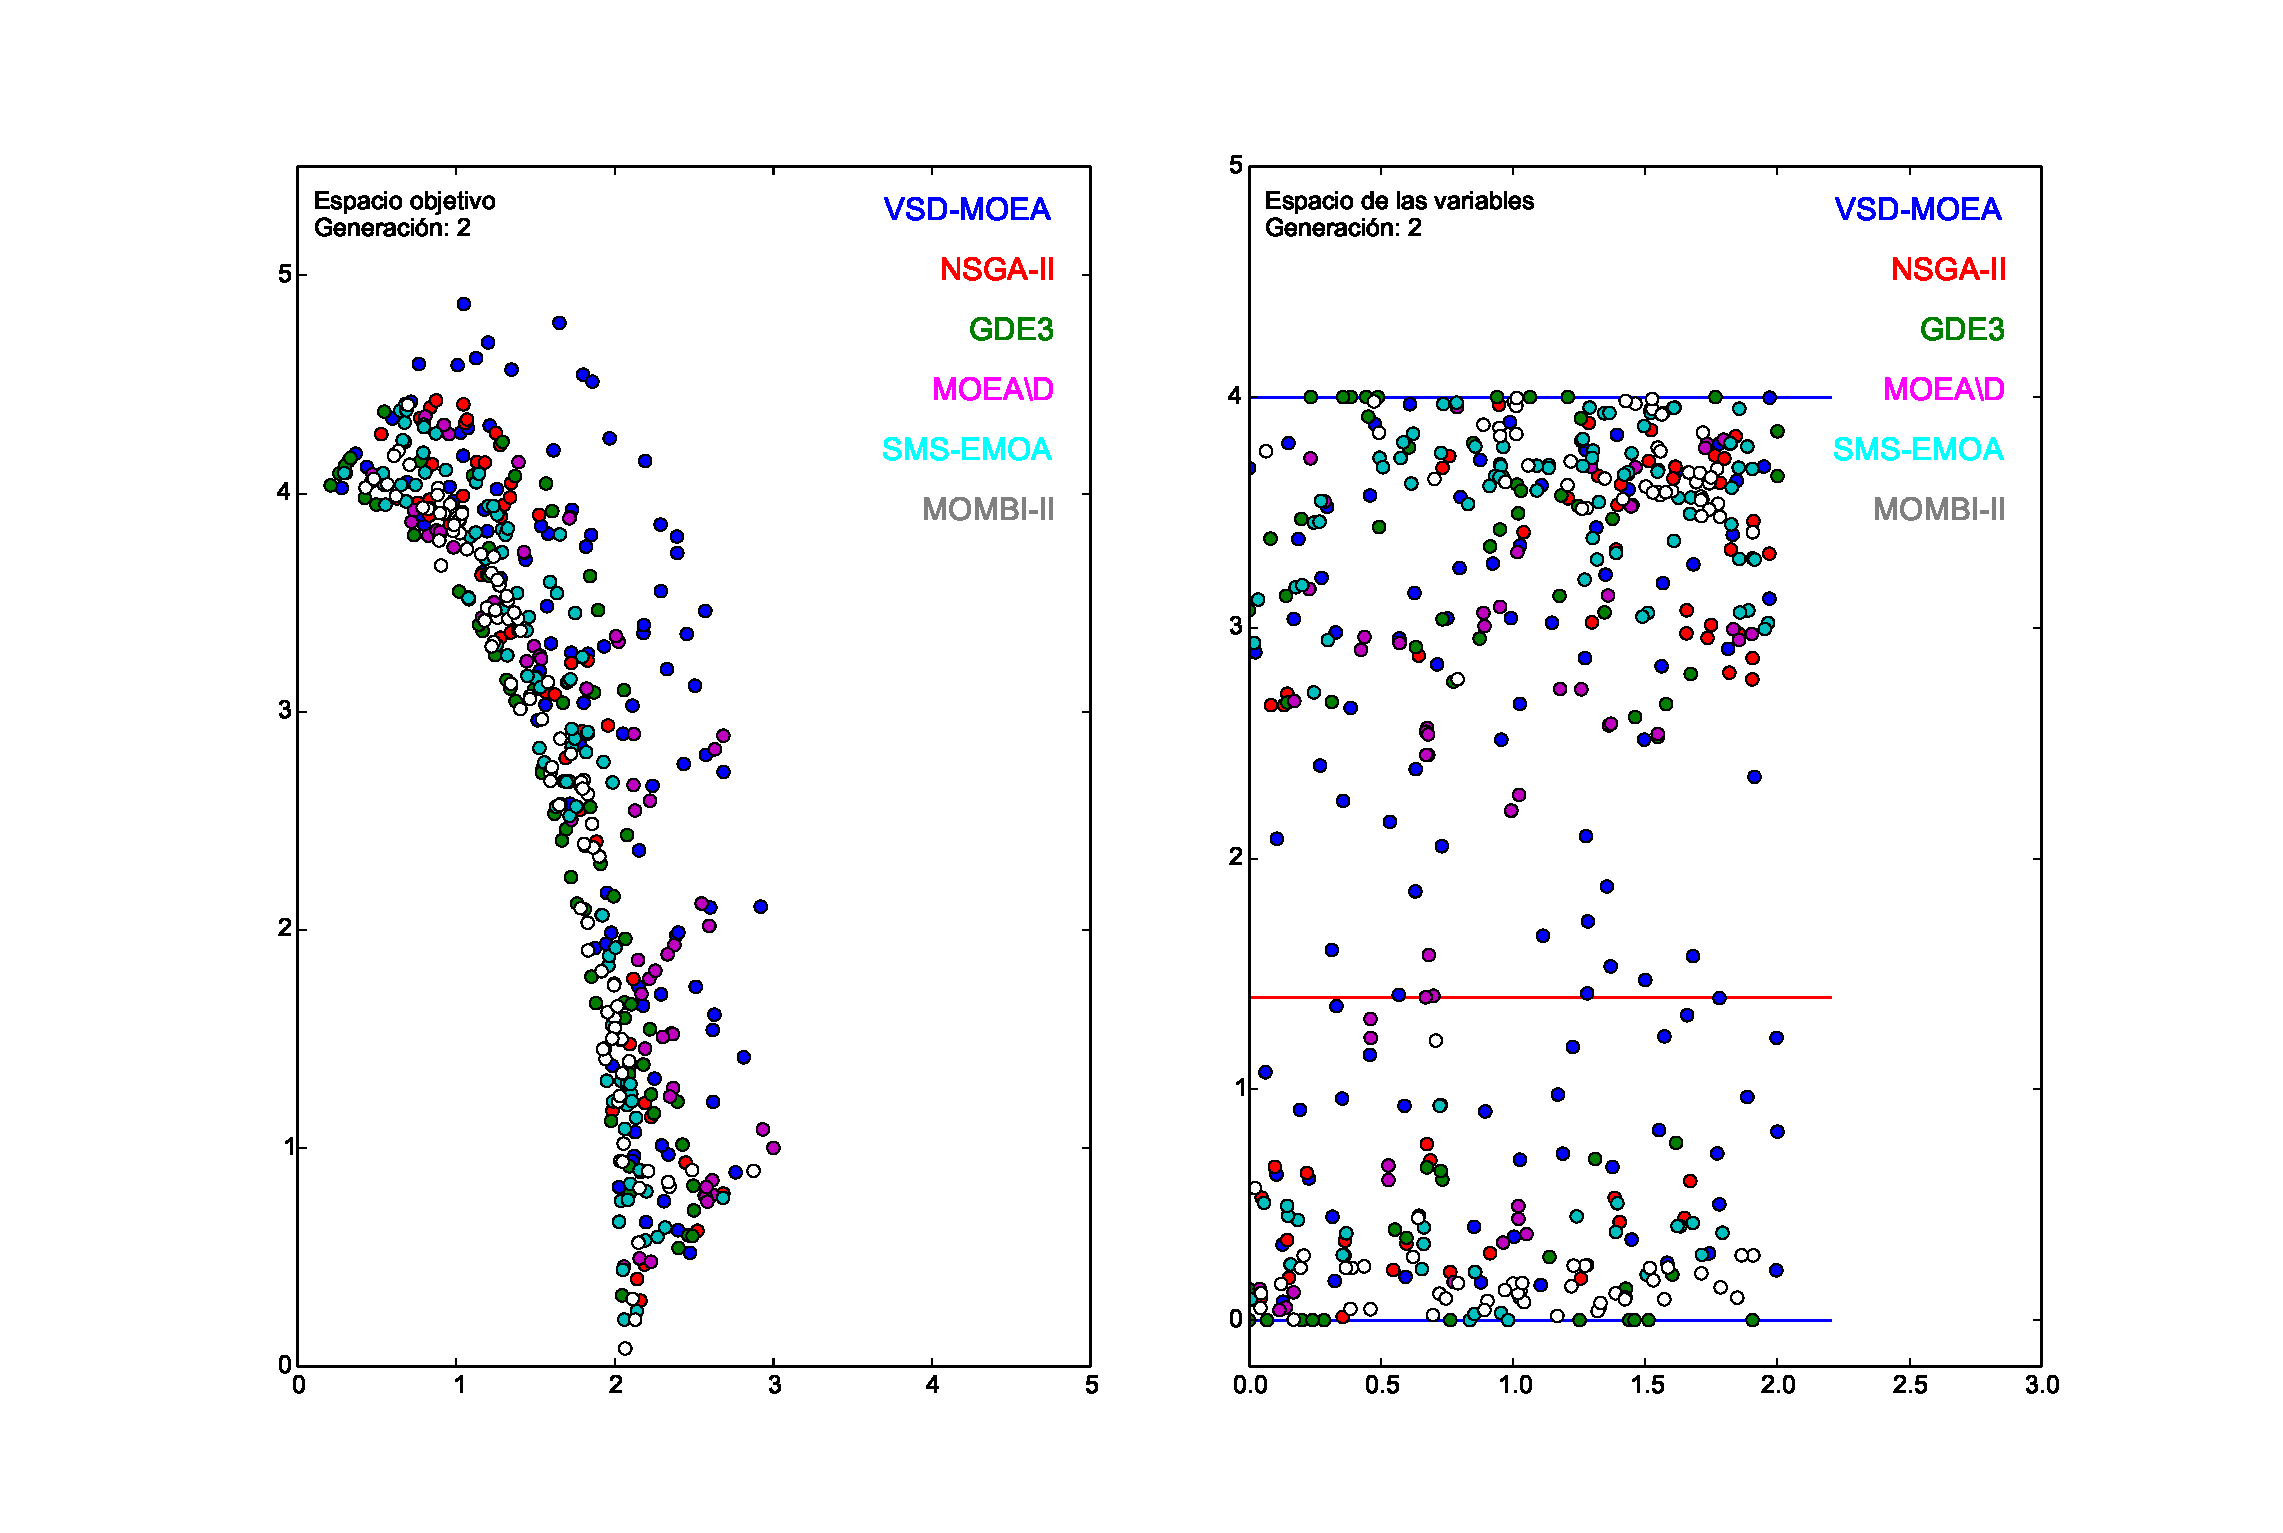
\includegraphics[scale=0.3]{Images/Simulacion_Algoritmo_1.eps}\\[0cm]%[-0.14cm] 
 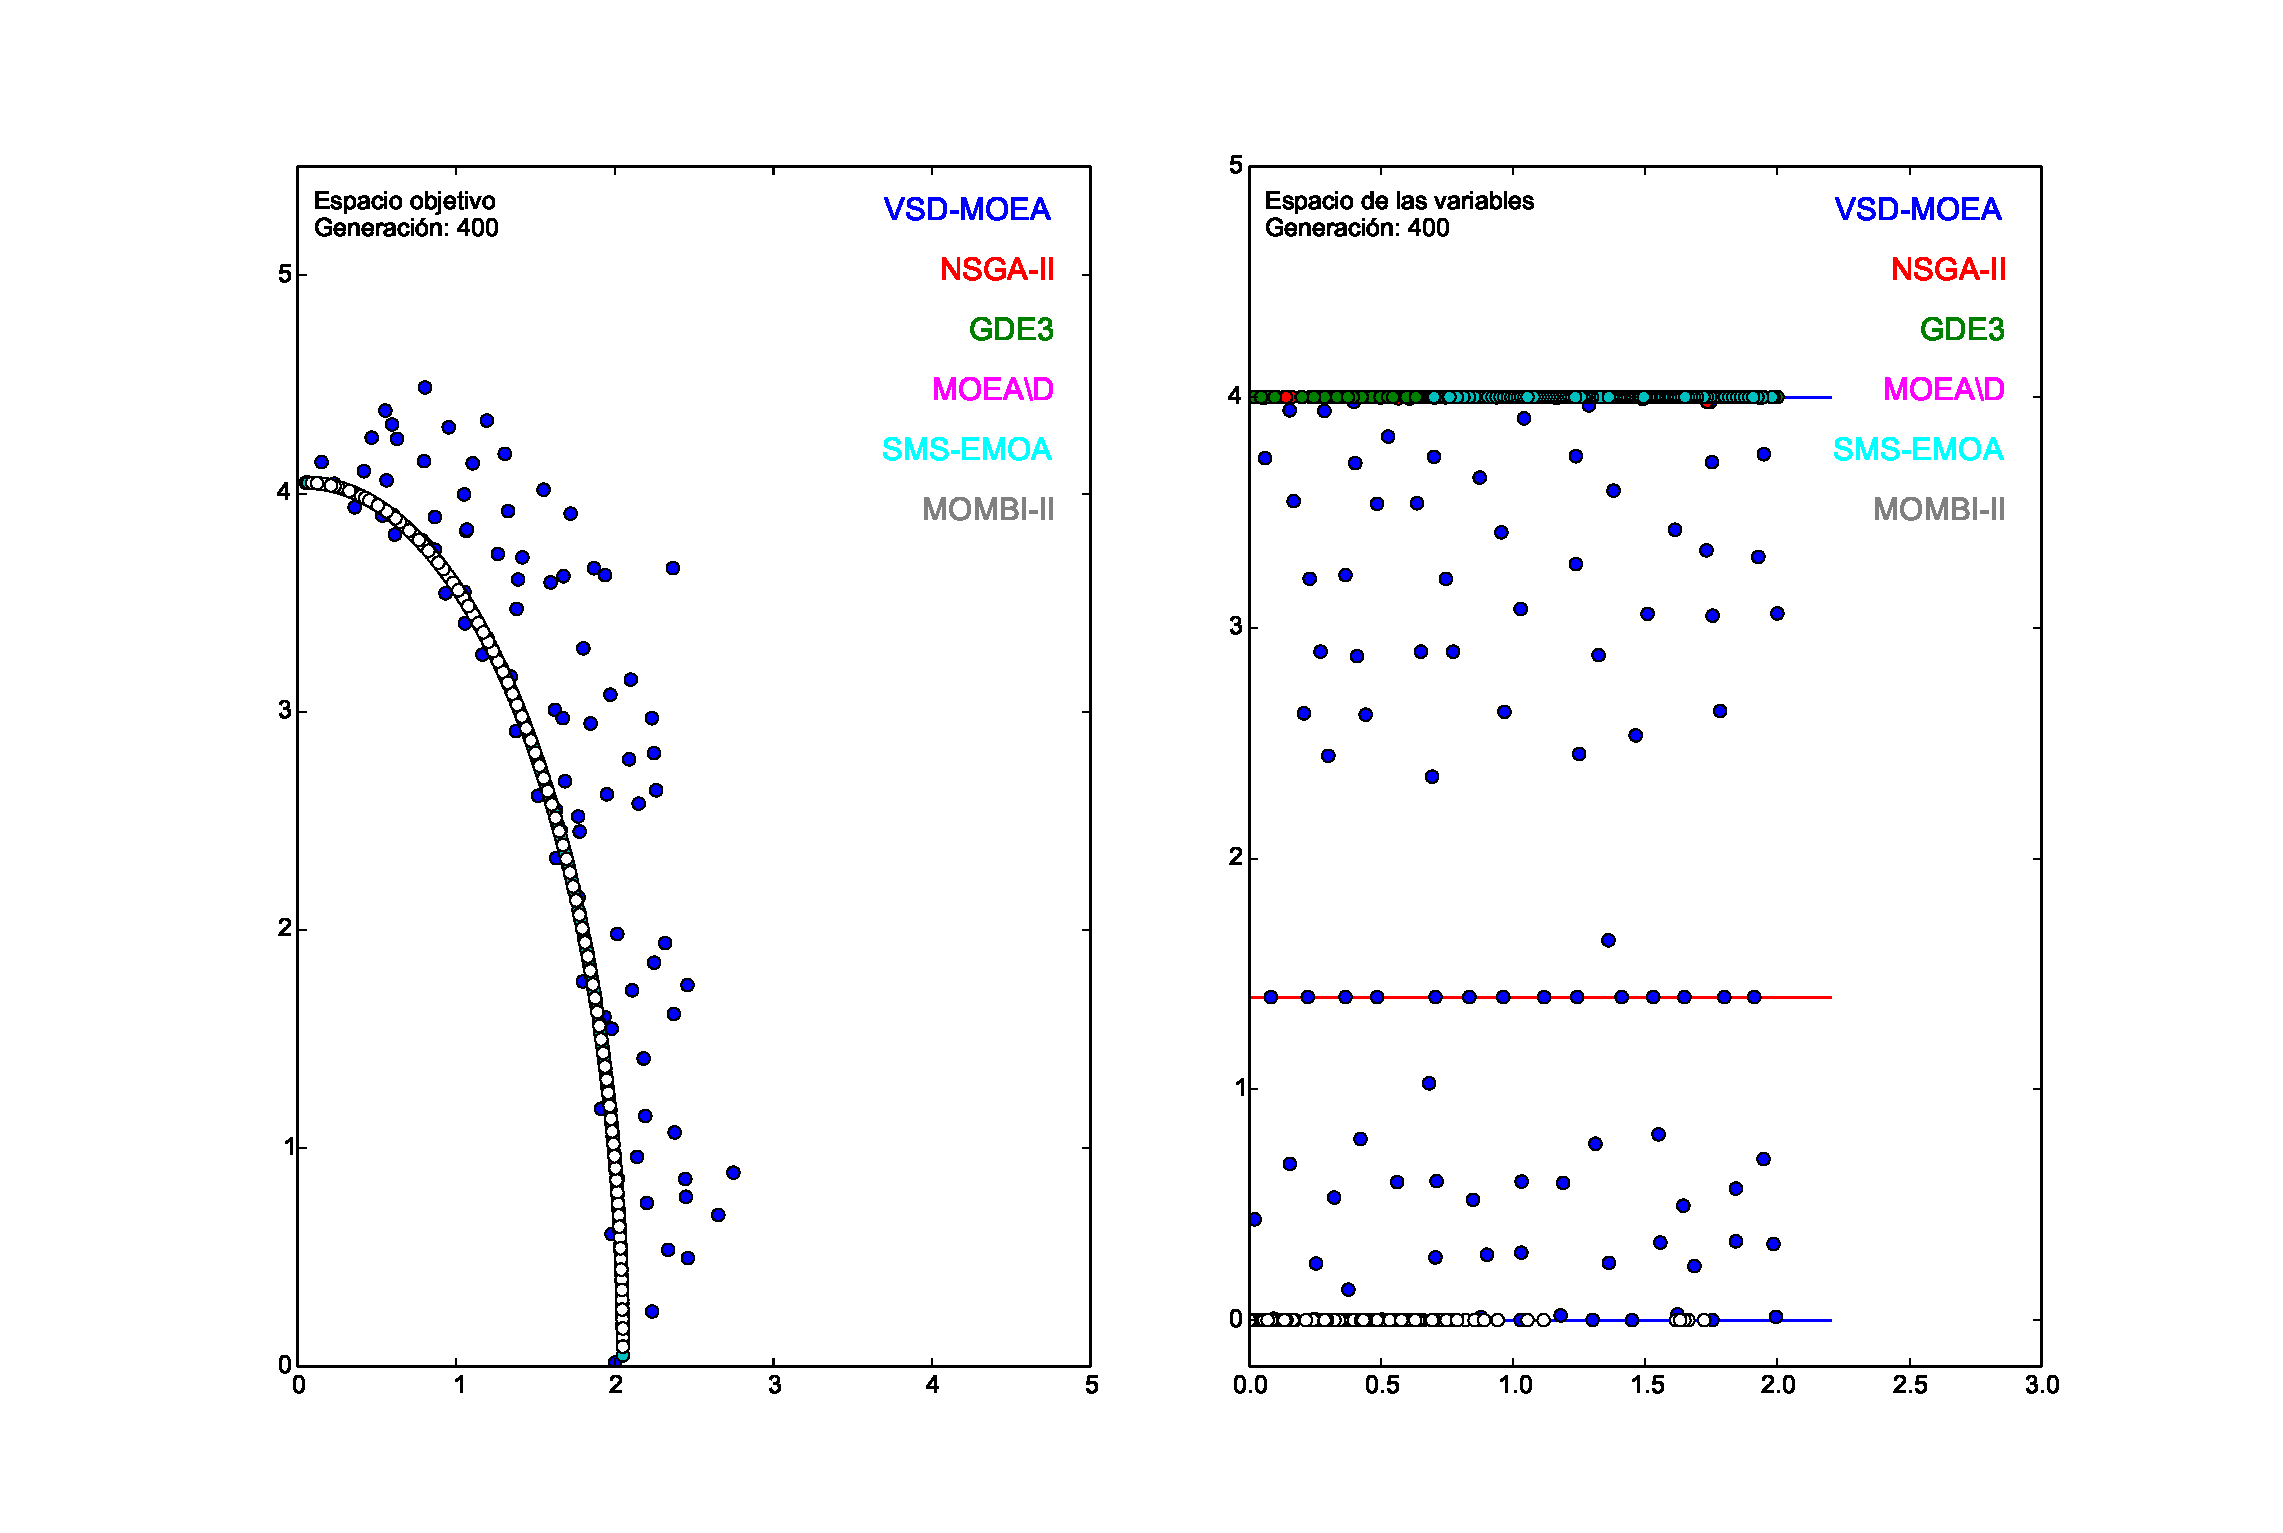
\includegraphics[scale=0.3]{Images/Simulacion_Algoritmo_4.eps}\\[0cm]%[-0.14cm] 
 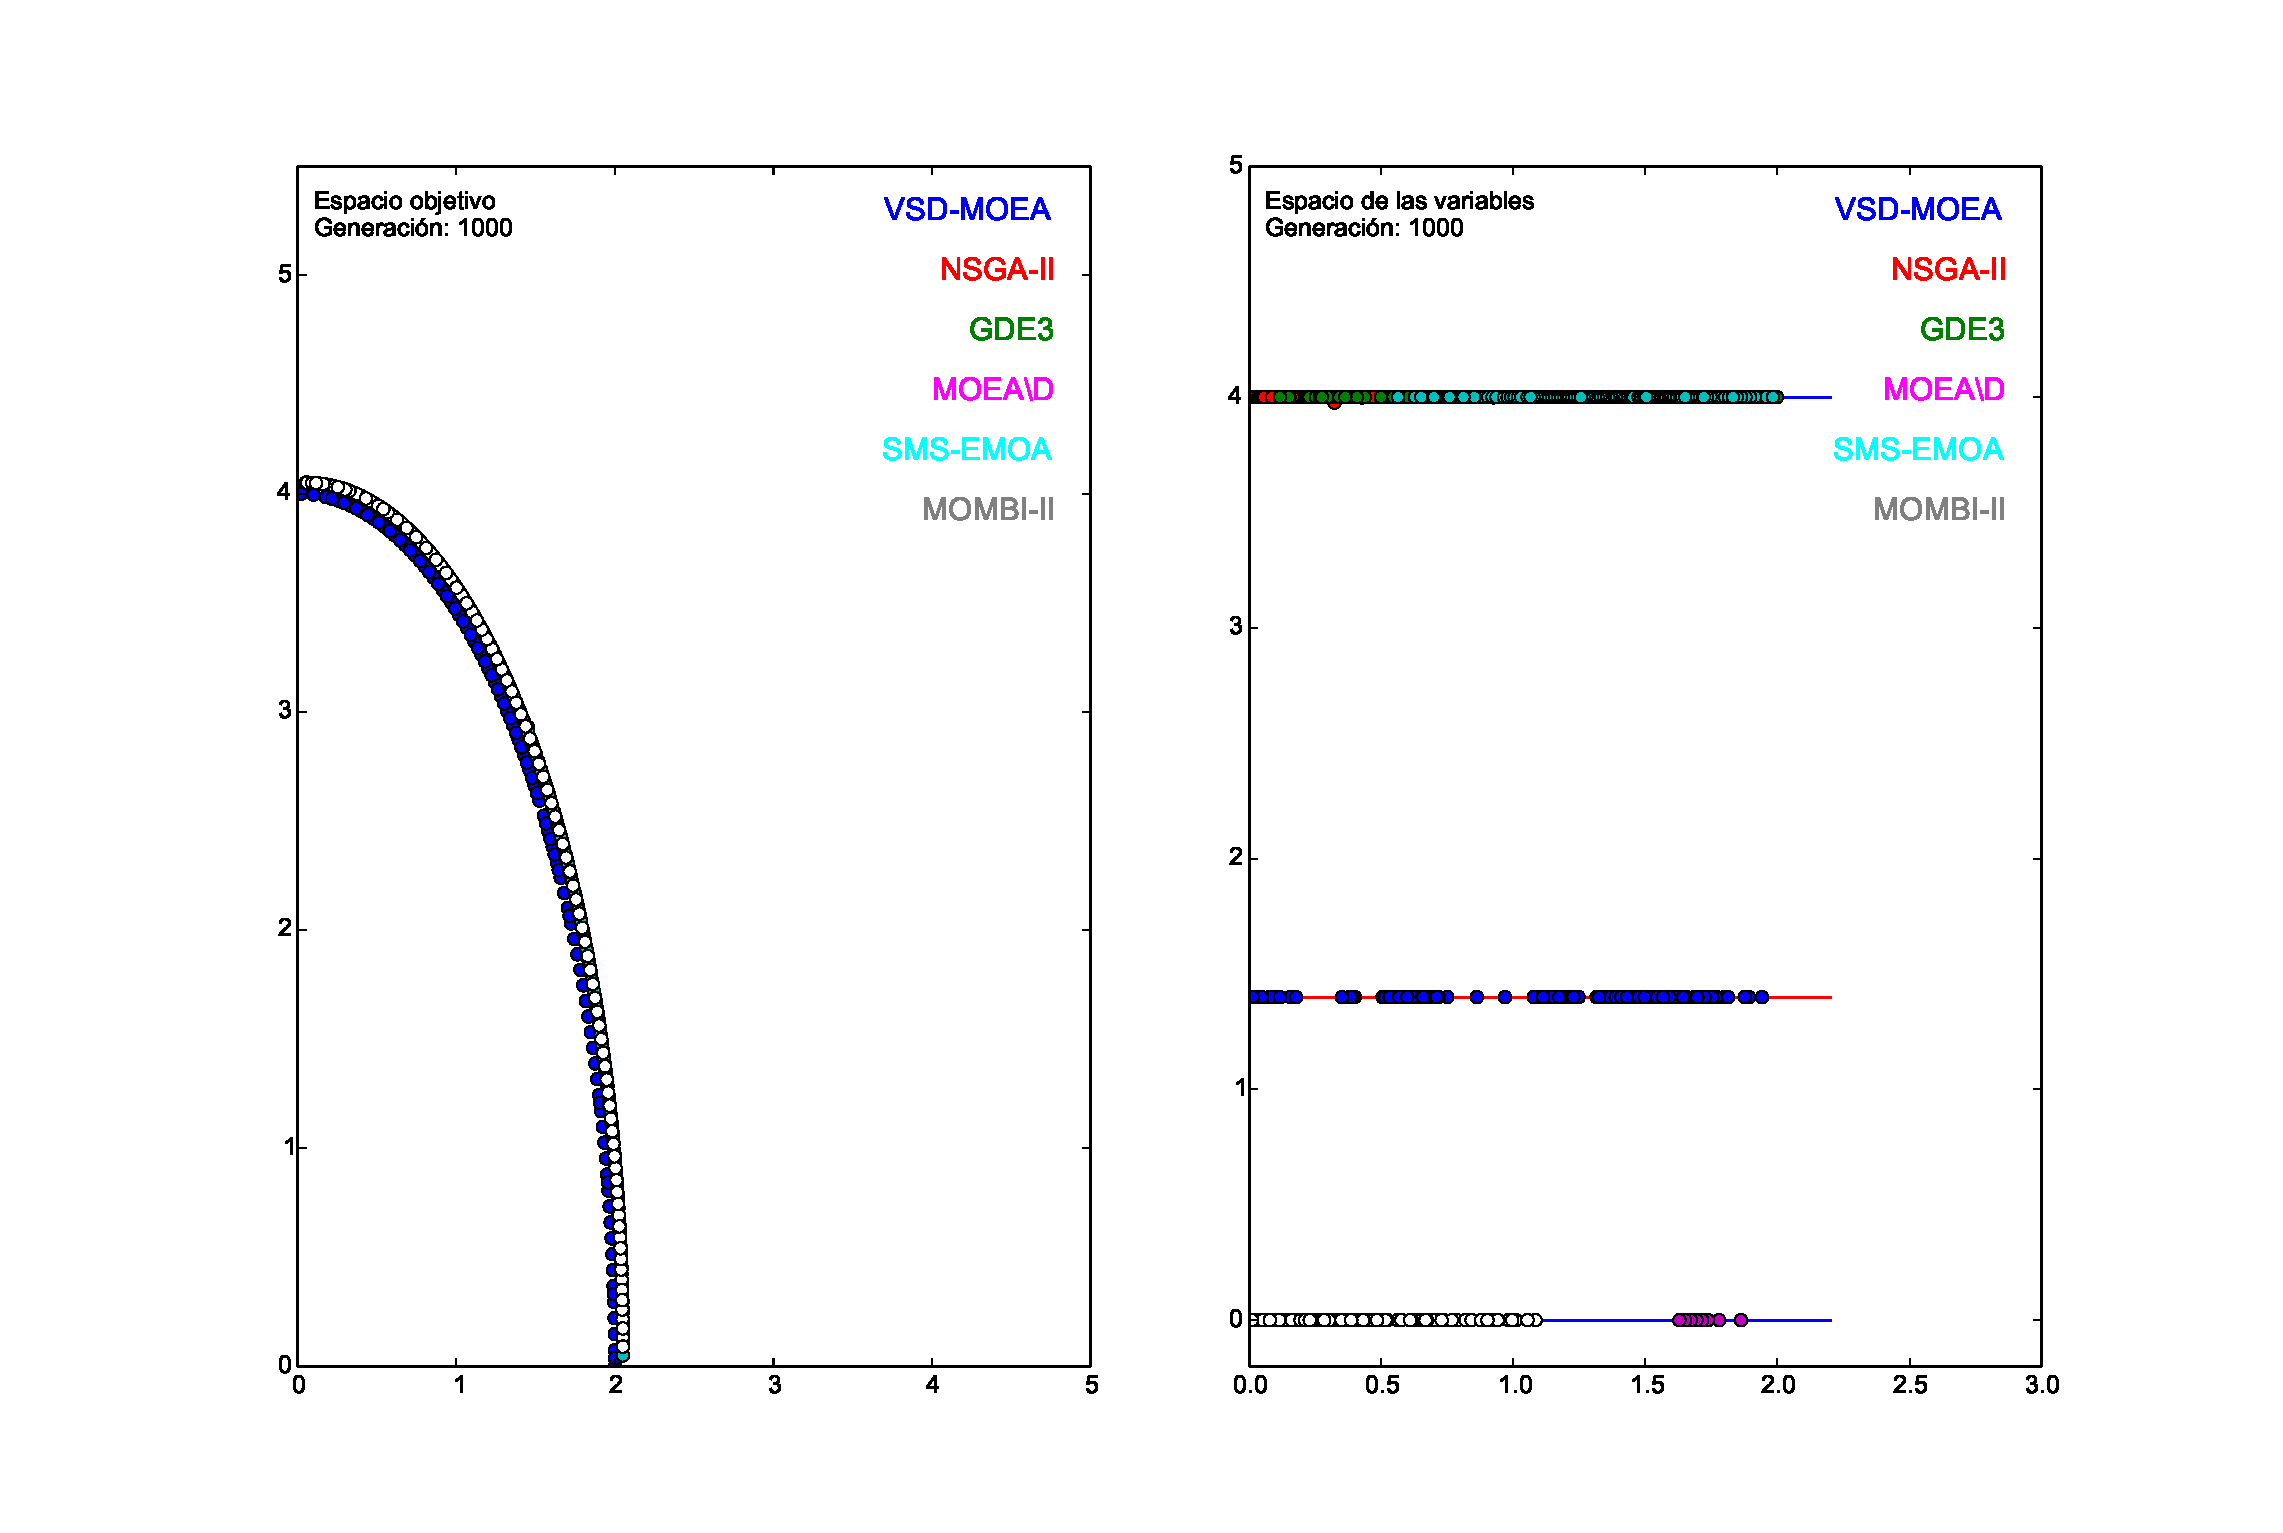
\includegraphics[scale=0.3]{Images/Simulacion_Algoritmo_5.eps}\\[0cm]%[-0.14cm] 
\end{tabular}
\caption{Performance of \MOEAS{} for the problems with three objectives considering three ranges of stopping criterion: short-term (first row), middle-term (second row) and long-term (third row).}\label{fig:Performance_time_3obj}
\end{figure}
